\section{General discussion}
\label{section:general_discussion}

The proposed pipeline for 3D point cloud video rendering gives good results comparing to raw data. It enables to move freely in the 3D created world of the scene which was the objective. The proposed registration approach to align the different views gives an acceptable visual result. The edge processing algorithm cancelled some of the edge effects. The colour correction improves the consistency even if it is still not perfect. The anti-flickering filter stabilises the image in the video stream. Together, all these three visual enhancement algorithms improve the quality of the point cloud video regarding what was done by \textit{LiveScan3D} \cite{kowalski_livescan3d:_2015}. However, using two cameras and point clouds for the 3D visualisation have some limitations.

'Holes' appear when an object or a body part passes in front of another part of the scene, see figure \ref{figure:00492_hole_red_background}. These 'holes' are like a shadow due to the time of flight technology. They are visible when the point of view is virtual and are in fact a lack of data. Because it is a lack of data, information of the static background often 'fills' this 'hole', see figure \ref{figure:00492_background_hole}. Using temporal information to reconstruct parts when information is missing was not tackled in this project but should be investigated in future work.

\begin{figure}[H]
\centering
  \begin{subfigure}[b]{0.48 \textwidth}
    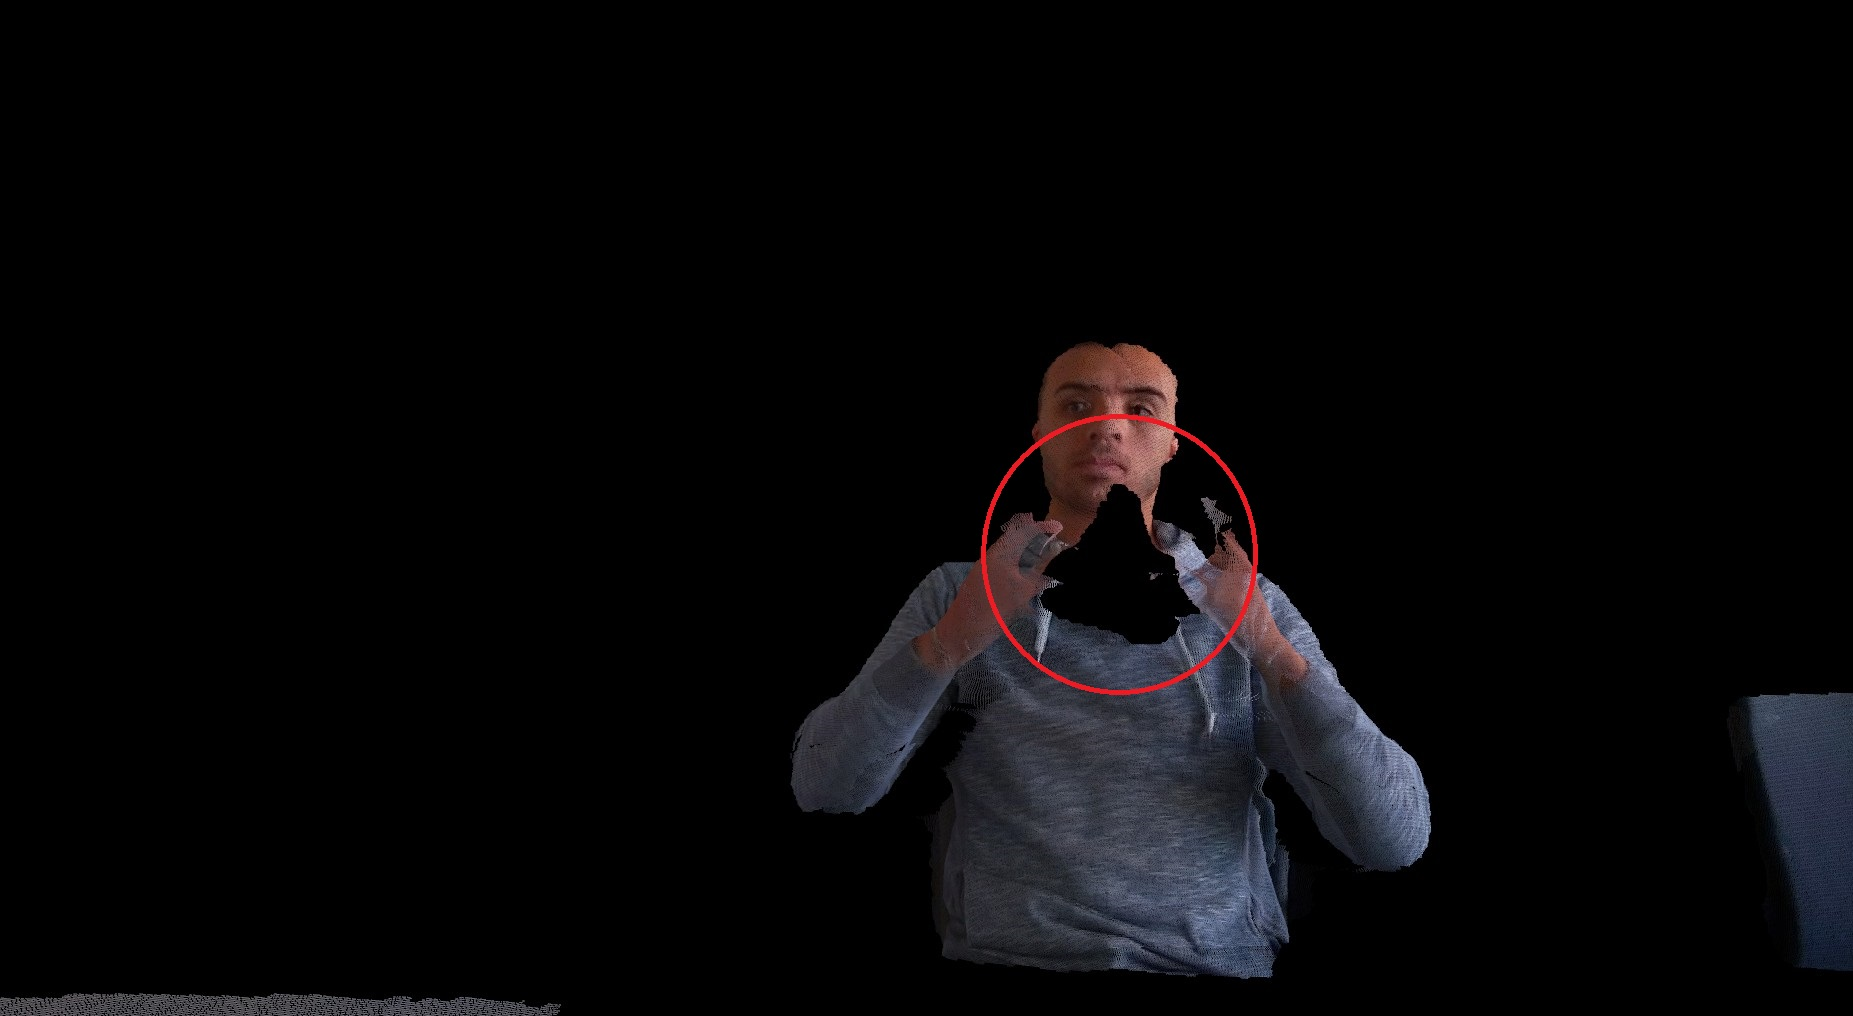
\includegraphics[width=\textwidth]{images/general_result/00492_hole_red.jpg}
    \caption{'Hole' visible in the middle of the body}
    \label{figure:00492_hole_red}
  \end{subfigure}
  \hfill
  \begin{subfigure}[b]{0.48 \textwidth}
    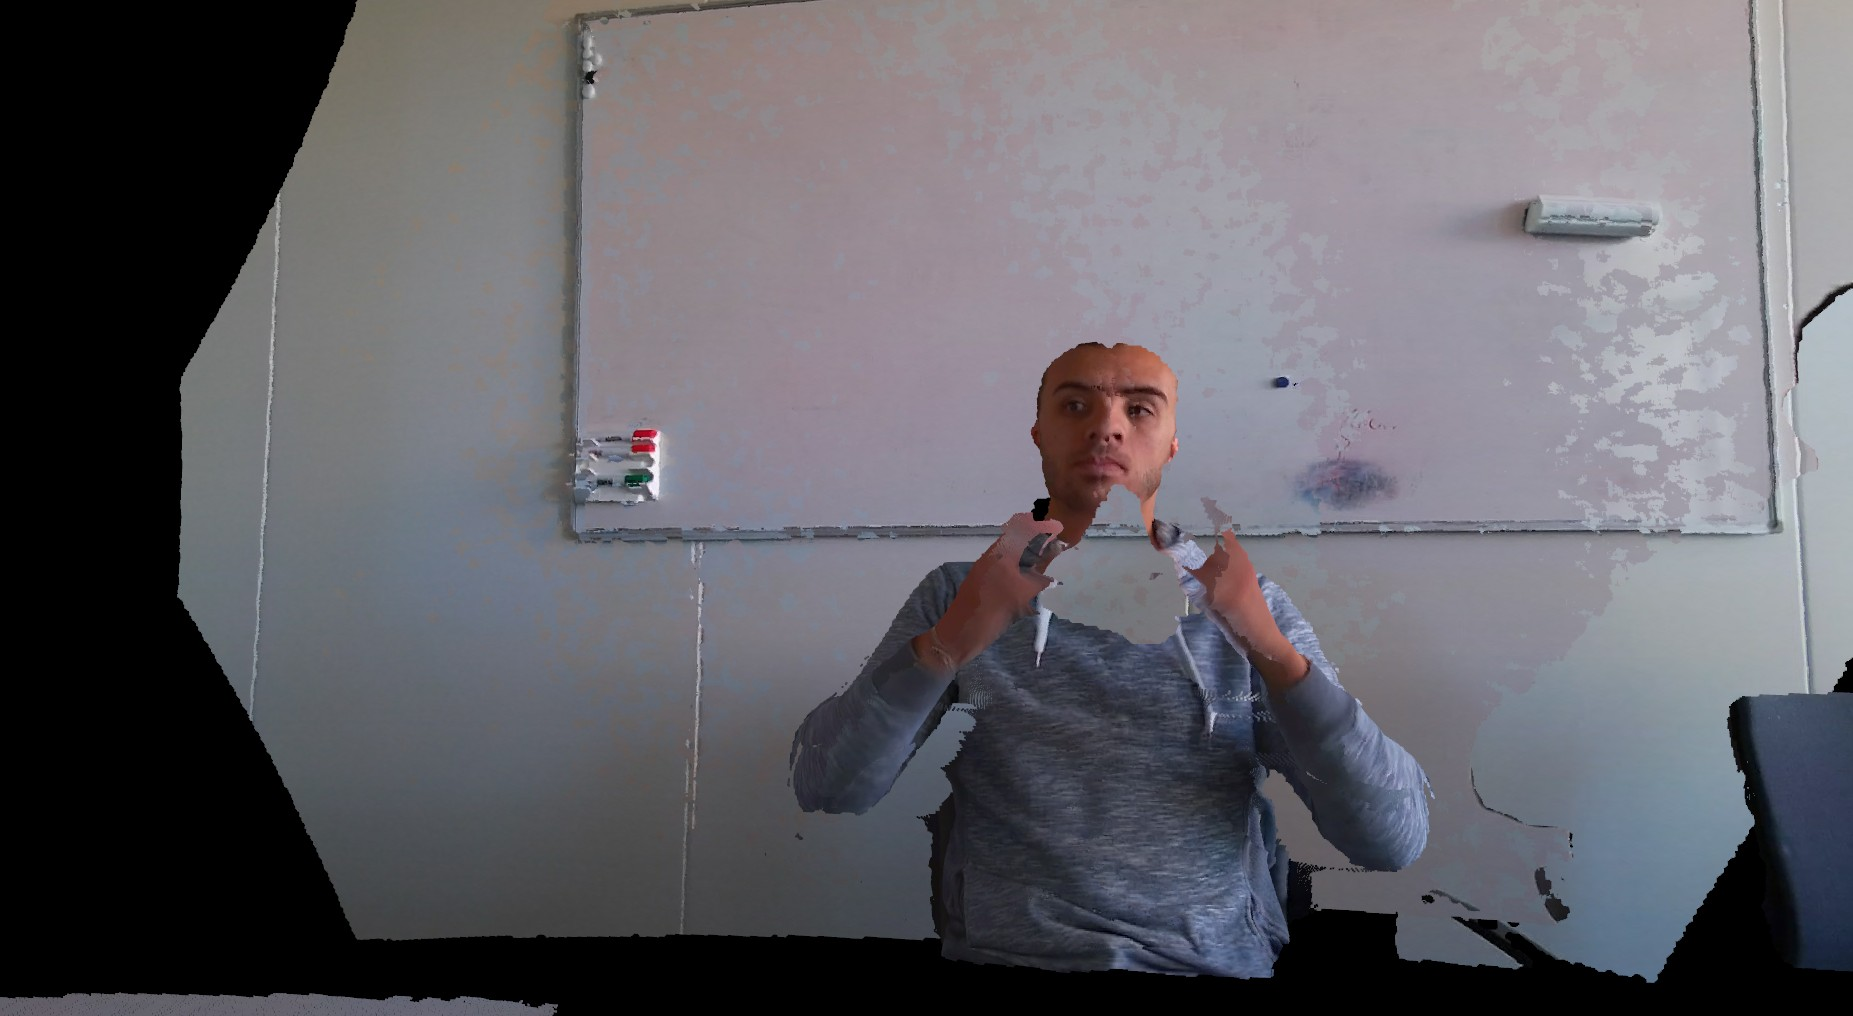
\includegraphics[width=\textwidth]{images/general_result/00492_background_hole.jpg}
    \caption{Static background visible in the middle of the body}
    \label{figure:00492_background_hole}
  \end{subfigure}
  \caption{Virtual viewpoint of the same scene with and without the static background. A 'hole' is visible in the middle of the body. In case of background, this hole is 'filled' with the background information. Hands doesn't look natural}
  \label{figure:00492_hole_red_background}
\end{figure}

Some body-parts do not look natural. Hands, for example, are not well reconstructed with point clouds created from the used Kinect camera. Using body part segmentation and a model of the hands could help to reconstruct such a body part.

As proof of concept, only two cameras were used in the pipeline. It improves the covered volume of the 3D reconstruction but it is not enough. 'Holes' are visible, some body parts are still only partially reconstructed. For a matter of time, increasing the number of cameras wasn't tried. It is surely a way to investigate to improve the rendering of the scene. Moreover, a study about where to place the camera in the room to optimise the covered reconstruction could be another path to increase this covered volume with a limited number of cameras.

The dense point cloud approach chosen in this thesis shows some limitation. Using raw point cloud results in a flickering effect. This effect is visually disturbing. Mesh instead of point cloud could be tried to determine if the reconstruction is more stable. Fitting data on a 3D model of a human body could also be a way to investigate in future works.

Time of flight technology of the used Azure Kinect cameras has also some limitation. In the case of glassy surfaces, the reconstruction is incomplete. The near-IR illumination seams to not reflect properly on this kind of surface depending on the incidence angle. Because the information of the depth is missing, the point cloud reconstruction of that kind of surface is incomplete. Some Logitech meeting rooms have some glassy wall and are therefore not well reconstructed, see figure \ref{figure:glass_wall_issue_red}. 

\begin{figure}[H]
    \centering
    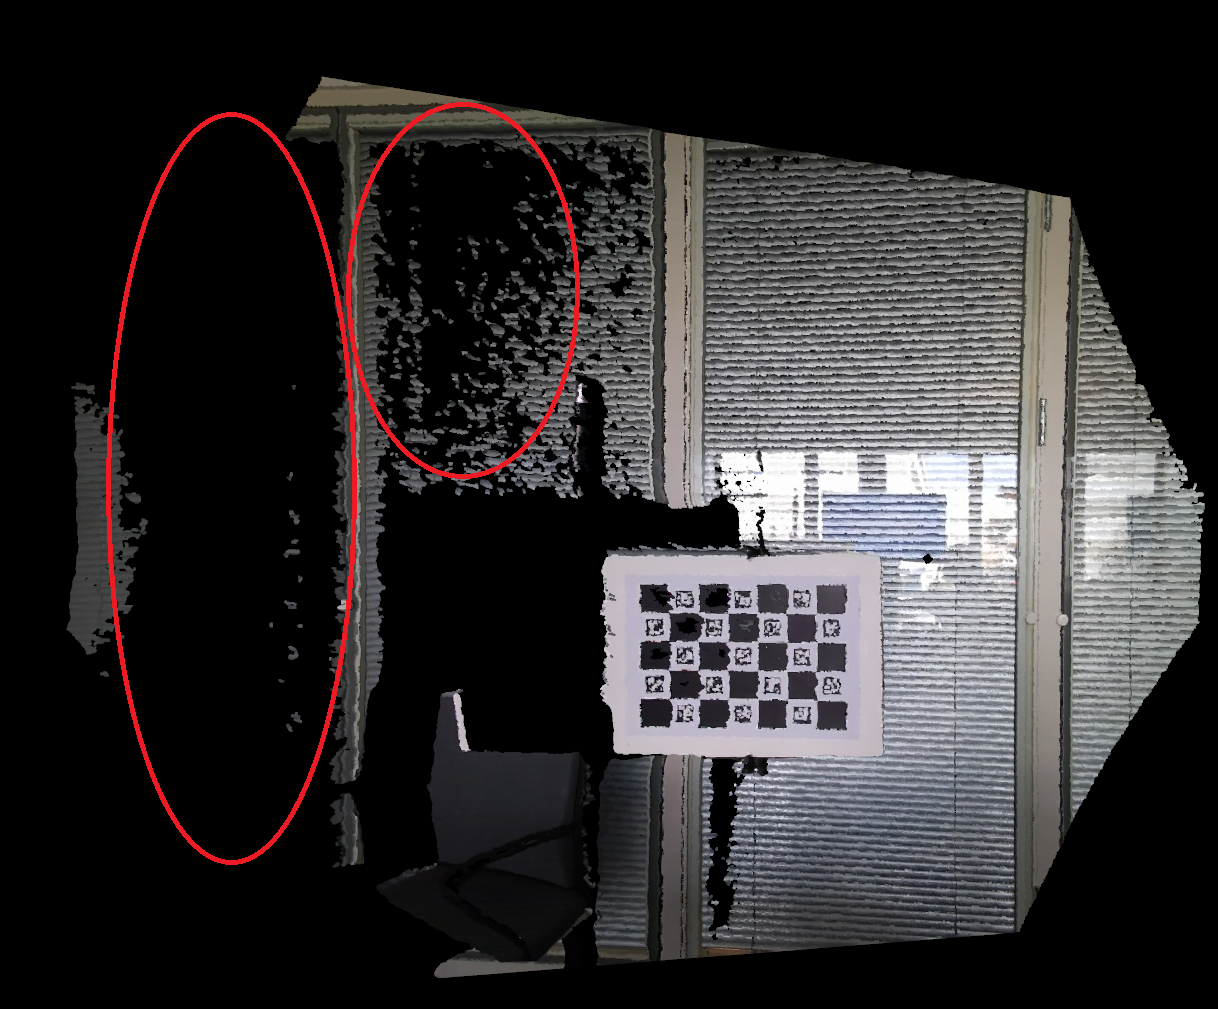
\includegraphics[width=0.45\textwidth]{images/general_result/glass_wall_issue_red.png}
    \caption{Reconstruction issue of the glassy wall}
    \label{figure:glass_wall_issue_red}
\end{figure}





% -limitaiton of th epoint lcoud approach


% -Static background: put image with it



